\section{Punto de Vista de función de Negocio}

El punto de vista de la cooperación de los procesos comerciales se utiliza para mostrar las relaciones de uno o más procesos comerciales entre sí y/o con su entorno. Puede utilizarse tanto para crear un diseño de alto nivel de los procesos empresariales dentro de su contexto como para proporcionar a un director operacional responsable de uno o más de esos procesos una visión de sus dependencias. Los aspectos importantes de la cooperación en los procesos empresariales son:

\begin{itemize}
	\item Relaciones causales entre los principales procesos comerciales de la empresa
	\item Mapeo de los procesos comerciales en las funciones comerciales
	\item Realización de servicios por procesos comerciales
	\item Uso de datos compartidos
\end{itemize}

Cada una de ellas puede considerarse un "subpunto de vista" del punto de vista de la cooperación en los procesos comerciales.

\subsection{Modelo de función de Negocio}
\begin{figure}[h!]
	\centering
	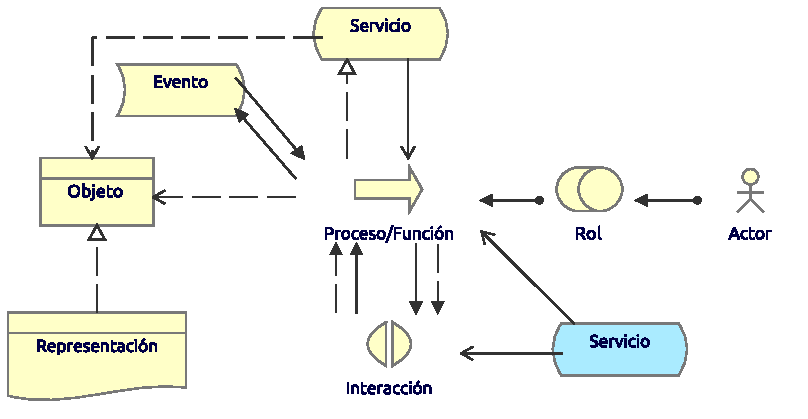
\includegraphics[width=.8\linewidth]{imgs/modelo/ProcesoNegocio}
	\caption{Modelo función de Negocio}
\end{figure}

Un proceso empresarial representa una secuencia de comportamientos empresariales que logra un resultado específico, como un conjunto definido de productos o servicios empresariales.
Un proceso de negocios describe el comportamiento interno realizado por un rol de negocios que se requiere para producir un conjunto de productos y servicios. Para un consumidor, los productos y servicios son relevantes y el comportamiento requerido es meramente una caja negra, de ahí la designación "interno".
Un proceso comercial complejo puede ser una agregación de otros procesos de grano más fino. A cada uno de ellos se le pueden asignar funciones más finas.
Existe una relación potencial de muchos a muchos entre los procesos de negocios y las funciones de negocios. En términos informales, los procesos describen algún tipo de "flujo" de actividades, mientras que las funciones agrupan las actividades según las aptitudes, los conocimientos, los recursos, etc. requeridos. Un proceso empresarial puede ser desencadenado por, o desencadenar, cualquier otro elemento de comportamiento empresarial (por ejemplo, un acto empresarial, un proceso empresarial, una función empresarial o una interacción empresarial). Un proceso empresarial puede acceder a objetos empresariales. Un proceso empresarial puede realizar uno o más servicios empresariales y pueden utilizar servicios comerciales (internos) o servicios de aplicación. Se puede asignar una función empresarial a un proceso empresarial para realizar este proceso manualmente. Un proceso empresarial automatizado puede realizarse mediante un proceso de aplicación. El nombre de un proceso empresarial debe indicar claramente una secuencia predefinida de acciones, y puede incluir la palabra "proceso". Ejemplos de ello son "adjudicar la reclamación", "incorporación de empleados", "proceso de aprobación" o "presentación de informes financieros". \\

Un objeto comercial representa un concepto utilizado dentro de un dominio comercial determinado. Un contrato representa una especificación formal o informal de un acuerdo entre un proveedor y un consumidor en el que se especifican los derechos y obligaciones asociados a un producto y se establecen parámetros funcionales y no funcionales para la interacción. Una representación representa una forma perceptible de la información que lleva un objeto comercial.

\clearpage
\subsection{Caso  de función de Negocio}
\begin{figure}[h!]
	\centering
	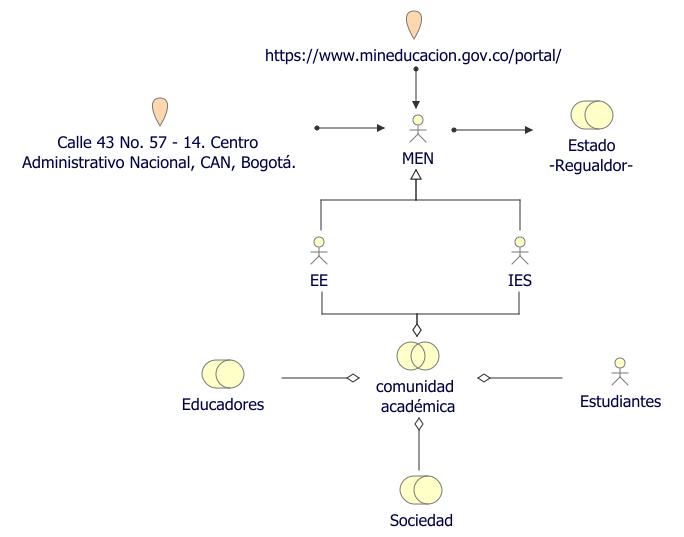
\includegraphics[width=.9\linewidth]{imgs/caso/negocio/organizacion}
	\caption{Caso función de Negocio}
\end{figure}
descripcion...
